\begin{frame}{Introdução}
A forma \alert{mais expressiva} com que os humanos exibem emoções é através de \alert{expressões faciais}. Os humanos detectam e interpretam faces e expressões faciais em uma cena com \alert{pouco ou nenhum esforço}. Ainda assim, o desenvolvimento de um sistema automatizado que realiza essa tarefa é bastante difícil \cite{fasel2003automatic}.

  \begin{figure}
    \centering
    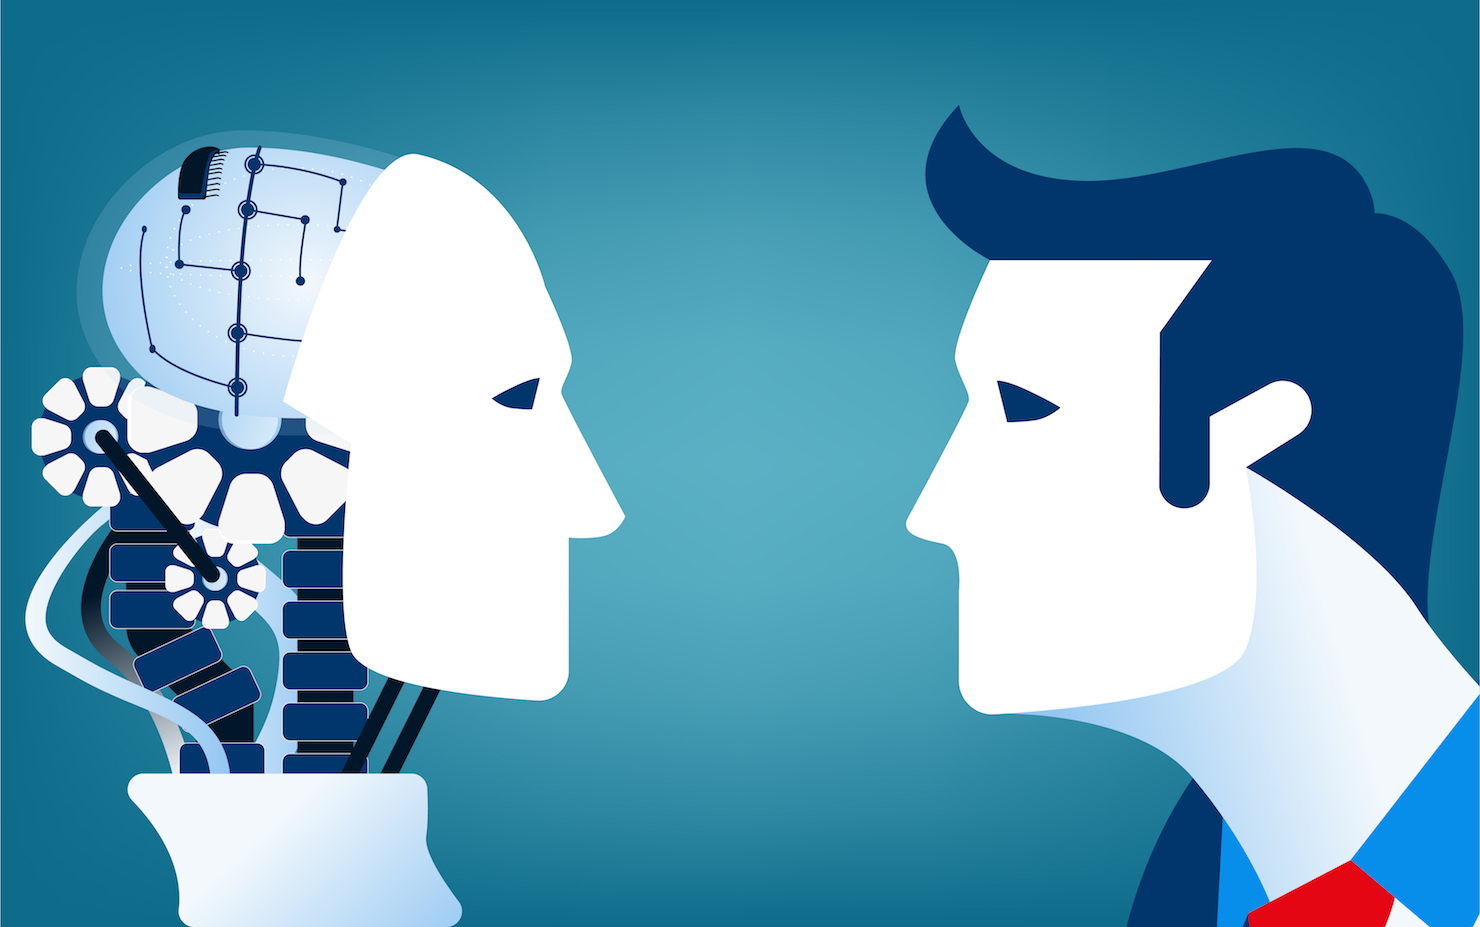
\includegraphics[scale=0.1]{img/human_vs_computer.jpeg}
    \caption{Reconhecimento de expressões faciais: homem vs máquina \cite{francis-school}.}
  \end{figure}

\end{frame}

\begin{frame}
\frametitle{Introdução - Universalidade das expressões faciais}

\begin{itemize}
    \item The Expression of Emotions in Man and Animals
    \begin{itemize}
        \item Universalidade das expressões faciais
        \item Emoções inatas
    \end{itemize}
    \item Emoções básicas
\end{itemize}

\begin{figure}[h!]
	\centering
	\begin{tabular}{@{}c@{}}
		\subfloat[Felicidade]{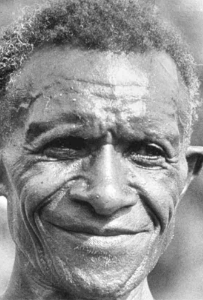
\includegraphics[width=0.23\linewidth]{img/happy_pe.png}}
		\subfloat[Tristeza]{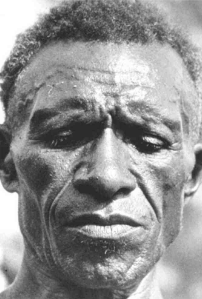
\includegraphics[width=0.23\linewidth]{img/sad_pe.png}}
		\subfloat[Raiva]{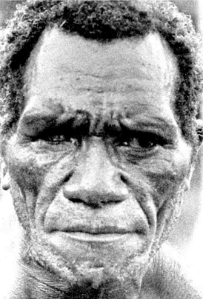
\includegraphics[width=0.23\linewidth]{img/angry_pe.png}}
		\subfloat[Nojo]{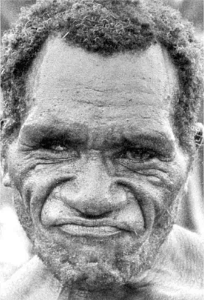
\includegraphics[width=0.23\linewidth]{img/disgust_pe.png}}
	\end{tabular}
	\caption{Expressões faciais de nativo do sul da Nova Guiné\cite{collins}}
\end{figure}

\end{frame}

\begin{frame}{Introdução - Aplicações}
  
\begin{columns}
    \begin{column}{0.4\textwidth}
      \begin{itemize}
            \item Comportamento do consumidor
            \item Estudo de usabilidade
            \item Teste de fármacos
            \item Muitas outras
        \end{itemize}
    \end{column}
    
    \begin{column}{0.6\textwidth}
        \begin{center}
            \begin{figure}[T]
                \label{fig:introduction_application}
            	\begin{tabular}{@{}c@{}}
            		\subfloat[Vitrine]{
            		    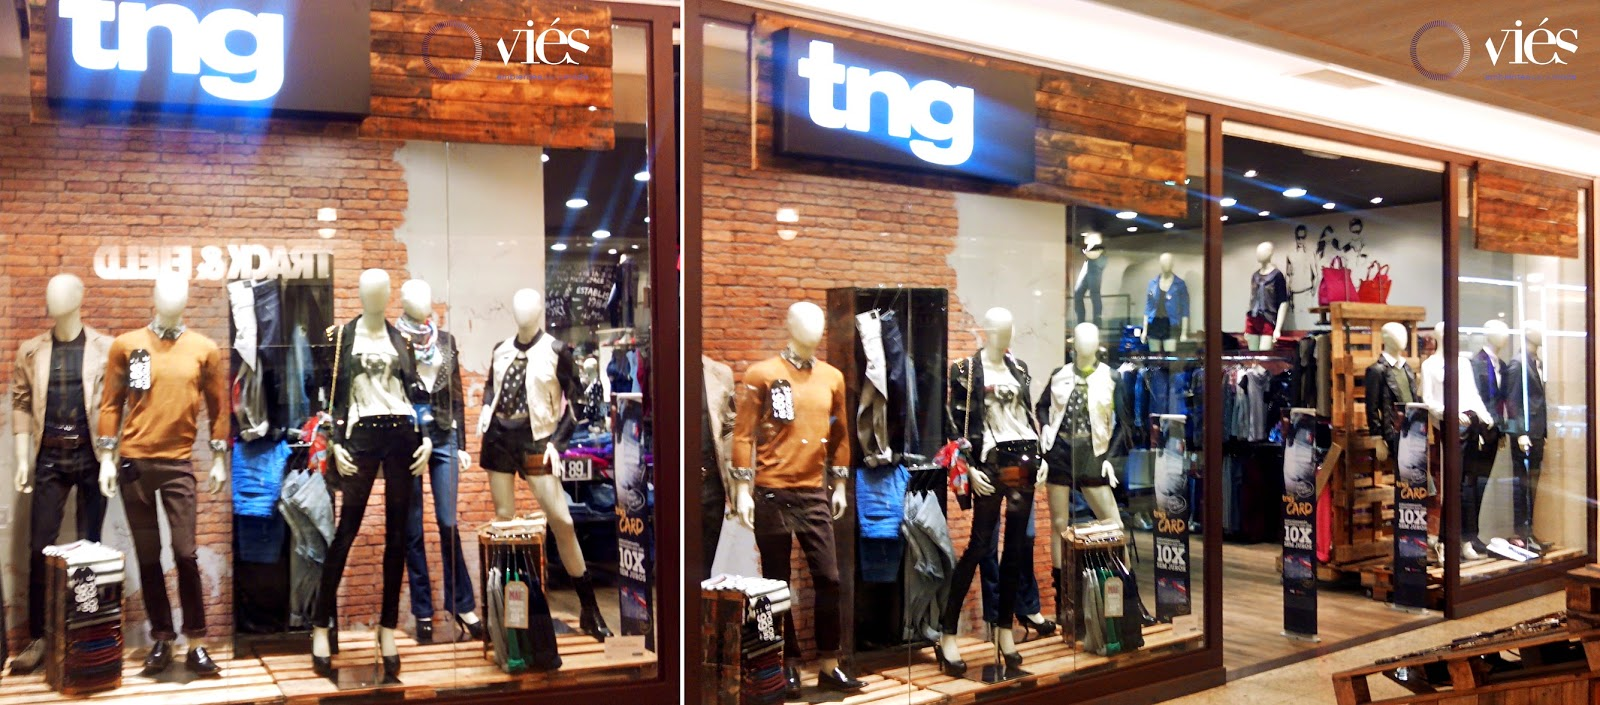
\includegraphics[width=1.0\linewidth]{img/vitrine.jpg}
            		  %  \caption{Consumer behavior \cite{showcase}}
            		}
            	\end{tabular}
            	
            	\begin{tabular}{@{}c@{}}
            		\subfloat[Usabilidade]{
            		    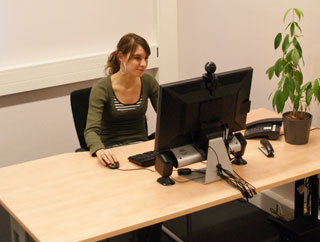
\includegraphics[width=0.5\linewidth]{img/usability-testing.jpg}
            		  %  \caption{Usability testing \cite{usability_testing}}
            		}
            		\subfloat[Fármacos]{
            		    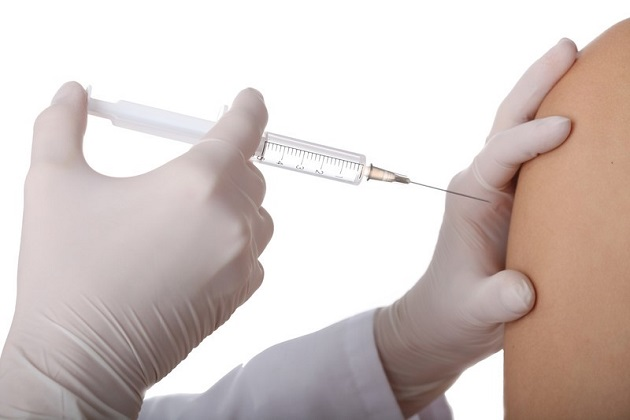
\includegraphics[width=0.5\linewidth, height=0.2754\textheight]{img/vacina.jpg}
            		  %  \caption{Drug testing \cite{drug_testing}}
            		}
            	\end{tabular}
            \end{figure}

        \end{center}
    \end{column}
\end{columns}  
  
\end{frame}

\setcounter{subfigure}{0}
\begin{frame}{Introdução}

Desafio: Classificação de expressões faciais baseados em imagens estáticas \textit{in the wild}.

\begin{figure}[h!]
    \label{fig:introduction_basic}
	\centering

	\begin{tabular}{@{}c@{}}
		\subfloat[Felicidade]{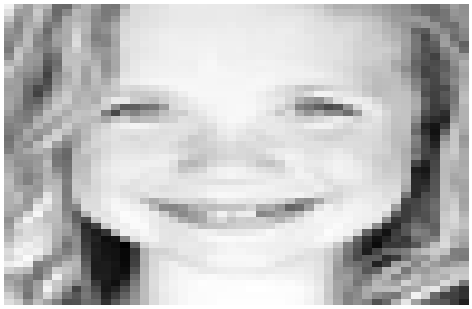
\includegraphics[width=0.20\linewidth,keepaspectratio]{img/sample_happy.png}} \quad
		\subfloat[Nojo]{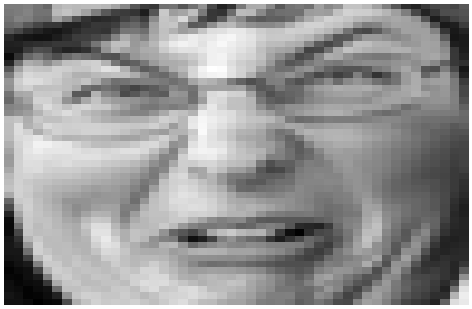
\includegraphics[width=0.20\linewidth, keepaspectratio]{img/sample_disgust.png}} \quad
		\subfloat[Tristeza]{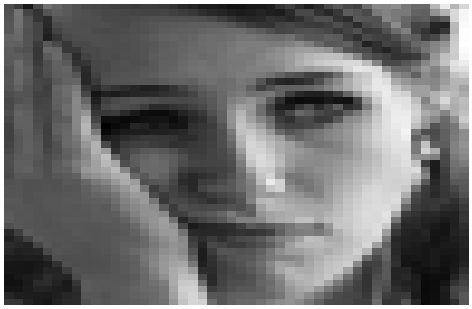
\includegraphics[width=0.20\linewidth, keepaspectratio]{img/sample_sad.png}}
	\end{tabular}

	\vspace{\floatsep}

  \begin{tabular}{@{}c@{}}
		\subfloat[Surpresa]{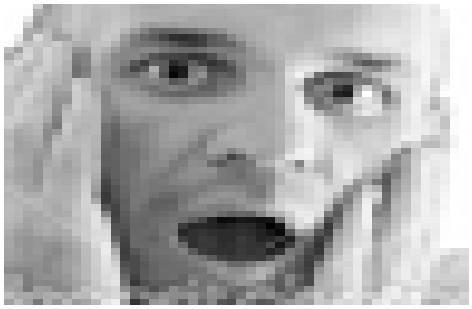
\includegraphics[width=0.20\linewidth, keepaspectratio]{img/sample_surprise.png}} \quad
  	\subfloat[Medo]{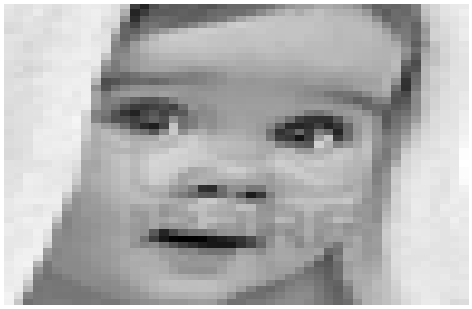
\includegraphics[width=0.20\linewidth, keepaspectratio]{img/sample_fear.png}} \quad
  	\subfloat[Raiva]{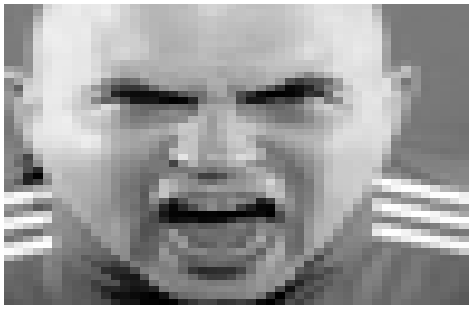
\includegraphics[width=0.20\linewidth, keepaspectratio]{img/sample_angry.png}} \quad
    \subfloat[Neutro]{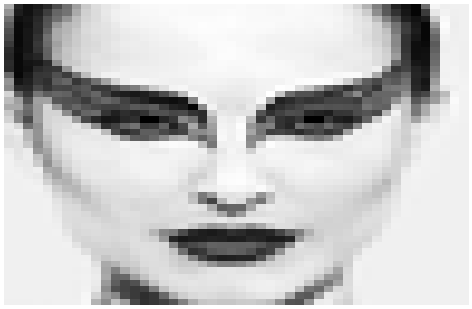
\includegraphics[width=0.20\linewidth, keepaspectratio]{img/sample_neutral.png}}
  \end{tabular}
  \captionof{figure}{Amostra da base de dados FER2013.}
\end{figure}
    
\end{frame}